\documentclass[a4paper,11pt]{article}

\usepackage{graphicx}
\usepackage[margin=2.8cm]{geometry}
\usepackage{wrapfig}
\usepackage[colorlinks=true,urlcolor=blue,linkcolor=black]{hyperref}
\usepackage{color}
\usepackage[english]{babel}
\usepackage{forloop}

\newenvironment{reqlist}{\par \medskip \noindent \begin{tabular}{cp{0.83\textwidth}r} \\[-24pt]}{\end{tabular}}
\newenvironment{subreqlist}{\begin{tabular}{cp{0.923\textwidth}r} \\[-24pt]}{\end{tabular}}
\newcommand\req{\\ \smallskip \smallskip \hspace{0.24cm} $\bullet$\hspace{-0.2cm} & }
\newcommand\subreq{\\ \smallskip \smallskip \hspace{0.5cm} -\hspace{-0.2cm} & }

\newcounter{num}
\newcommand\effort[1]{\mbox{(\forloop{num}{0}{\value{num} < #1}{$\star$})}}


\begin{document}

\thispagestyle{empty}

\noindent
\hrulefill \vspace{6pt}

\noindent

\includegraphics[viewport=8 8 185 55]{figures/eth_logo_black} \hfill

\includegraphics[trim=0 0 2 0]{figures/disco-logo-col} \hspace{-6pt} \vspace{-6pt}

\noindent \hrulefill \vspace{4pt}

\hfill Prof.\ R.\ Wattenhofer

\noindent BA/SA: \bigskip

\noindent \textbf{\LARGE Simulating Bitcoin's Network Topology} \bigskip

\noindent Bitcoin is a decentralized dynamic peer-to-peer network. The security of the transactions is dependent on the information propagation time, hence the network topology is important for Bitcoin' s  operation. The protocol implements a specific way of connecting new peers to the existing network to ensure the graph structure resembles that of a random graph while obfuscating the network topology to protect against various attacks (e.g. eclipse attack).

\bigskip

\begin{wrapfigure}{r}{6.5cm}
	\vspace{-0.5cm}
	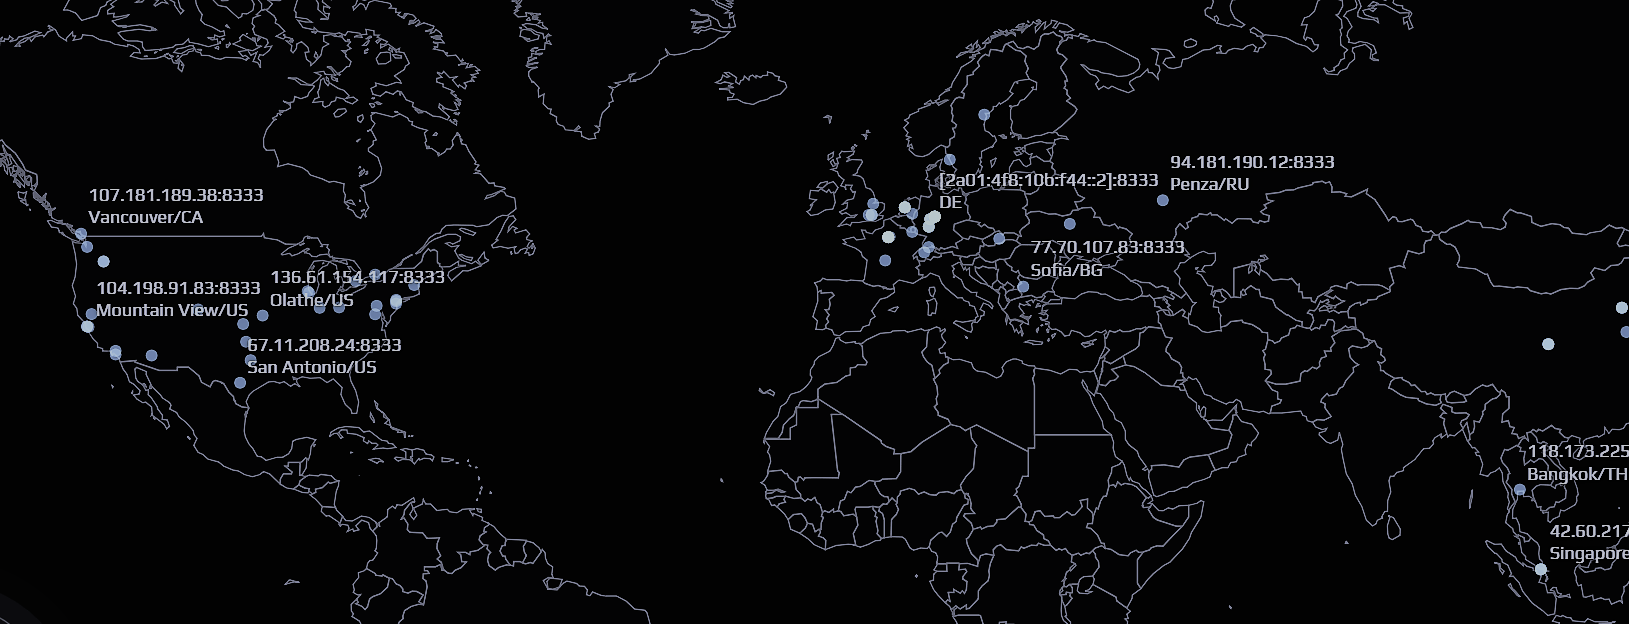
\includegraphics[width=6.5cm]{figures/bitcoin_topology.png}
\end{wrapfigure}

\noindent In this thesis, we will have a close look at the connection strategy of the bitcoin network and evaluate its fairness properties regarding the interests of all bitcoin miners. Our goal is to identify weaknesses in the running system and propose a more robust solution.
\bigskip

\noindent \textbf{Requirements:} The nature of this project is mostly practical; hence, programming experience is an advantage. There will be weekly meetings with your supervisors to discuss progress and open questions.
\bigskip

\noindent \textbf{Interested? Please contact us for more details!}

\subsection*{Contacts}
\begin{itemize}
	\item Georgia Avarikioti: \href{mailto:Georgia Avarikioti <zetavar@ethz.ch>}{\texttt{zetavar@ethz.ch}}, ETZ G95
	\item Roland Schmid: \href{mailto:Roland Schmid <roschmi@ethz.ch>}{\texttt{roschmi@ethz.ch}}, ETZ G94
\end{itemize}

% The part following this line is usually not part of the bait but rather meant as part of the assigmnent for a student when he starts the thesis.
\newpage

\subsection*{Detailed Project Outline}
We denote the following primary tasks mandatory (on the right side you find a rough estimate for the time that we allocate to the respective task):
\begin{reqlist}
	\req understand bitcoin's connection strategy in detail & \effort{2}
	\req defining metrics for simulation & \effort{2}
	\req evaluate how to implement the simulation best & \effort{1}
	\req write simulation of the broadcasting algorithm used by bitcoin & \effort{4}
	\req compare simulation to real data as far as one finds any & \effort{3}
	\req come up with a different connection strategy "X" & \effort{4}
	\req implement connection strategy in simulation & \effort{2}
	\req compare connection strategy with bitcoin's current broadcasting algorithm on fairness and efficency & \effort{2}
	\req report and presentation & \effort{2}
\end{reqlist}

\subsection*{Extensions}
\noindent Apart from these requirements, we can think of plenty of ways to extend the \textit{bitcoins broadcasting algorithm} with cool features. Of course, you may add your own ideas to this non-exhaustive enumeration:
\begin{itemize}
	\item realtime simulation plots
	\item simulate multiple different broadcasting algorithms
\end{itemize}

\end{document}
